%%%%%%%%%%%%%%%%%%%%%%%%%%%%%%%%%%%%%%%%%%%%%%%%%%%%%%%%%%%%%%%%%%%%
%% I, the copyright holder of this work, release this work into the
%% public domain. This applies worldwide. In some countries this may
%% not be legally possible; if so: I grant anyone the right to use
%% this work for any purpose, without any conditions, unless such
%% conditions are required by law.
%%%%%%%%%%%%%%%%%%%%%%%%%%%%%%%%%%%%%%%%%%%%%%%%%%%%%%%%%%%%%%%%%%%%

\documentclass[
  digital, %% This option enables the default options for the
           %% digital version of a document. Replace with `printed`
           %% to enable the default options for the printed version
           %% of a document.
  twoside, %% This option enables double-sided typesetting. Use at
           %% least 120 g/m² paper to prevent show-through. Replace
           %% with `oneside` to use one-sided typesetting; use only
           %% if you don’t have access to a double-sided printer,
           %% or if one-sided typesetting is a formal requirement
           %% at your faculty.
  table,   %% This option causes the coloring of tables. Replace
           %% with `notable` to restore plain LaTeX tables.
  nolof,     %% This option prints the List of Figures. Replace with
           %% `nolof` to hide the List of Figures.
  nolot,     %% This option prints the List of Tables. Replace with
           %% `nolot` to hide the List of Tables.
  %% More options are listed in the user guide at
  %% <http://mirrors.ctan.org/macros/latex/contrib/fithesis/guide/mu/fi.pdf>.
]{fithesis3}
%% The following section sets up the locales used in the thesis.
\usepackage[resetfonts]{cmap} %% We need to load the T2A font encoding
\usepackage[T1,T2A]{fontenc}  %% to use the Cyrillic fonts with Russian texts.
\usepackage[ruled,vlined,linesnumbered,noresetcount]{algorithm2e}
\usepackage[
  main=english, %% By using `czech` or `slovak` as the main locale
                %% instead of `english`, you can typeset the thesis
                %% in either Czech or Slovak, respectively.
  english, german, russian, czech, slovak %% The additional keys allow
]{babel}        %% foreign texts to be typeset as follows:
%%
%%   \begin{otherlanguage}{german}  ... \end{otherlanguage}
%%   \begin{otherlanguage}{russian} ... \end{otherlanguage}
%%   \begin{otherlanguage}{czech}   ... \end{otherlanguage}
%%   \begin{otherlanguage}{slovak}  ... \end{otherlanguage}
%%
%% For non-Latin scripts, it may be necessary to load additional
%% fonts:
\usepackage{paratype}
\def\textrussian#1{{\usefont{T2A}{PTSerif-TLF}{m}{rm}#1}}
%%
%% The following section sets up the metadata of the thesis.
\thesissetup{
    date          = \the\year/\the\month/\the\day,
    university    = mu,
    faculty       = fi,
    type          = bc,
    author        = Martin Geletka,
    gender        = m,
    advisor       = Mgr. Samuel Pastva,
    title         = {Implementation of Cylindrical Algebraic Sub-decomposition},
    TeXtitle      = {Implementation of Cylindrical Algebraic Sub-decomposition},
    keywords      = {Polynomial zeros, Real algebraic geometry, Polynomial projection, Computational algebra, Real algebraic geometry},
    TeXkeywords   = {Polynomial zeros, Real algebraic geometry, Polynomial projection, Computational algebra, Real algebraic geometry},
    abstract      = {The goal of my bachelor thesis is to study and implement the algorithm of Cylindrical Algebraic Sub-decomposition.  The algorithm is used as the primary tool to study of semi-algebraic sets, which have practical use in research of continuous and hybrid models. 
Need of this thesis rest in the actual state of available implementations. These implementations are outdated or only included in commercial tools as Maple.
 Because of that the final application will be available as an open source library and used for further research of semi-algebraic sets.},
    thanks        = {I would like to express my sincerest gratitude to my supervisor, Mgr.
Samuel Pastva., for his guidance and the lots of invaluable advice he gave me during the
composition of this thesis.},
    bib           = example.bib,
}
\usepackage{makeidx}      %% The `makeidx` package contains
\makeindex                %% helper commands for index typesetting.
%% These additional packages are used within the document:
\usepackage{paralist} %% Compact list environments
\usepackage{amsmath}  %% Mathematics
\usepackage{amsthm}
\usepackage{amsfonts}
\usepackage{url}      %% Hyperlinks
\usepackage{markdown} %% Lightweight markup
\usepackage{listings} %% Source code highlighting
\usepackage{amssymb}
\usepackage{chngcntr}

\lstset{
  basicstyle      = \ttfamily,%
  identifierstyle = \color{black},%
  keywordstyle    = \color{blue},%
  keywordstyle    = {[2]\color{cyan}},%
  keywordstyle    = {[3]\color{olive}},%
  stringstyle     = \color{teal},%
  commentstyle    = \itshape\color{magenta}}
\usepackage{floatrow} %% Putting captions above tables
\floatsetup[table]{capposition=top}
\begin{document}
\chapter*{Introduction}
\addcontentsline{toc}{chapter}{Introduction}
The algorithm for cylindrical algebraic decomposition (CAD) was primarily invented in order to do a quantifier elimination over the reals. But nowadays it is considered as a general tool in the real algebraic geometry for studying subsets of $R^n$, that can be described by polynomial equations and inequalities (semi-algebraic sets).

The CAD algorithm as the tool for describing this semi-algebraic sets is often too powerful, because it produces much of the redundant information, that we do not need in the final application. The problem is that the CAD algorithm solves the complex problem of the decomposition of the $R^n$ into the regions, over which a given set of polynomials have a constant sign. These produce plenty of the result regions, which has no volume and often are unnecessary in the final application. That can be solved by the restriction of the result dimension. The algorithm with this restriction is often called as sub-CAD or in the specific case when we restrict only to the regions with volume in the final dimension as the full-dimensional CAD.

The goal of my thesis is to study possible changes to the basic Collins CAD algorithm  \citetitle{Arnon:1984:CAD:2054.2069}, which will lead to solving only sub-CAD and more specifically full-dimensional CAD. Then I apply these changes in the implementation of the CAD algorithm, which produce only full-dimensional regions. 
\newline
TODO spojit s contextom do jednej kapitoly a tu hodit state of art
\newline
This implementation will be open source and executable on Java Virtual Machine (JVM), because of the current unavailability of such application.

The thesis is divided into five main chapters. In the first chapter, I research the available implementation of the CAD algorithm and tools I used in my implementation. In the second chapter, I introduce a necessary background of CAD algorithm and then I formally define CAD, sub-CAD and full-dimensional CAD problem.
In the third chapter, I formally describe the CAD problem and introduce possible changes to the Collins implementation, which we can apply when we want to solve only sub-CAD or full-dimensional CAD problem. In the fourth chapter, we describe the implemented algorithm for full-dimensional CAD problem. And in the fifth chapter, we compare our implementation with other nowadays available implementations of CAD and sub-CAD problem. The final chapter concludes the outcome of this thesis.





%% We will define several mathematical sectioning commands.
\newtheorem{theorem}{Theorem}[section] %% The numbering of theorems
                               %% will be reset after each section.
\newtheorem{lemma}[theorem]{Lemma}         %% The numbering of lemmas
\newtheorem{corollary}[theorem]{Corollary} %% and corollaries will
                               %% share the counter with theorems.
\theoremstyle{definition}
\newtheorem{definition}{Definition}
\theoremstyle{remark}
\newtheorem*{remark}{Remark}

\counterwithin{definition}{chapter}

\chapter{Background and context}
The algorithm of cylindrical algebraic decomposition (CAD) was discovered by George E. Collins in 1973 and two years later published in his work \citetitle{10.1007/3-540-07407-4_17}. The paper describes the CAD method, which is much more efficient than the previous methods for a qualifier eliminations\cite{10.1007/3-540-07407-4_17}. The CAD algorithm became later also a powerful technique not only in the qualifier eliminations, but also in the real algebraic geometry for studying semi-algebraic sets and in many other fields, including robot motion planning\cite{LaValle:2006:PA:1213331},
epidemic modelling\cite{epidemicModeling} and theorem proving\cite{10.1007/978-3-642-32347-8_1}.

On the other hand, because of the high complexity of CAD algorithm, it is often replaced by other heuristics methods, when the number of input polynomials is too high.

The problem is that CAD usually produces far more information than required to solve the underlying problem\cite{Wilson2014}. We often want only a subset of a CAD sufficient to solve a particular problem. The algorithm, which solve only this problem is called sub-CAD. The primary focus of this thesis is to implement such changes in the method of the basic Collins CAD algorithms, which enables to solve this sub-CAD problem. 

After I did the research of available implementations of CAD and sub-CAD algorithm, I found out that nowadays there are only a few open-source implementations of CAD and none of the sub-CAD problem.

Possibly the first open source implementation which offers CAD algorithm is QEPCAD (Quantifier Elimination by Partial Cylindrical Algebraic Decomposition)
\footnote{
  See the documentation available at: \url{https://www.usna.edu/Users/cs/wcbrown/qepcad/B/QEPCAD.html}.
}. It is an interactive command-line program written in C language. The disadvantages of this open source application are that it does not implement the layered algebraic sub-decomposition and from information available at its web-pages, user documentation was last updated on 31 July 2002. Moreover, this implementation has not any version control repository and only a few active users, so it would be tough to collaborate on this project.

Other available implementation of CAD algorithm offers CARL(Computer Arithmetic Library),
\footnote{
  See the documentation available at: \url{https://smtrat.github.io/carl/classcarl_1_1CAD.html}
}
, which is an open source library implemented in C++. Although this implementation is available at the GitHub repository, it does not supports any implementations for the sub-CAD problem.
The only usable implementations of CAD algorithm runnable on JVM(Java Virtual Machine) and also implementing the sub-CAD are available in commercial tools like Maple 
\footnote{
See the Maple documentation available at: \url{https://www.maplesoft.com/support/help/maple/view.aspx?path=RegularChains\%2FSemiAlgebraicSetTools\%2FCylindricalAlgebraicDecompose}.
}
or Wolfram Mathematica 
\footnote{
  See the Wolfram Mathematica documentation available at: \url{https://reference.wolfram.com/language/ref/CylindricalDecomposition.html}.
}.

After my research of the state of art of CAD and sub-CAD implementations, I deduce there is a need for modern open source tool for the sub-CAD algorithm, which is the  topic of this thesis.

\chapter{Preliminaries and Definitions}
In this chapter, we firstly introduced notation and definitions used throughout this thesis. We used it to make a formal description of the problem of cylindrical algebraic decomposition. And finally, we describe and define a more specific version of this problem, which is a layered algebraic sub-decomposition.
\section{Polynomial definition and its characteristics}
Firstly we formulate the definition of the univariate polynomial, and it's elementary characteristics.
\begin{definition}{\textbf{Univariate polynomial}}
\newline
Univariate polynomial of degree $n$ over the ring $R$ is a function in the form:
\begin{align*}
p(x) =  \sum_{i=0}^n a_ix^i;\ \ \  a_i \in R, a_n \neq 0 
\end{align*}
The elements $a_0, a_1 .. a_n$ are called the coefficients of the polynomial $p$. Especially the coefficient $a_0$ is called constant coefficient and $a_n$ leading coefficient of the polynomial $p$.
\newline\newline
The set of all polynomial over ring $R$ is called the ring of the polynomials over $R$, and we represent it with symbol $R[x]$.
\end{definition}


After defining univariate polynomial, we describe some naming of some characteristics of the polynomials. The specific cases of the polynomials, which we use overall thesis,  are zero, constant and irreducible polynomial.  
\begin{definition}
Polynomial $f$ is called \textbf{zero polynomial} if all its coefficient equals to zero. All other polynomials are then called non-zero polynomial.
\end{definition}

\begin{definition}
Polynomials, which coefficient are all equal zero except the constant coefficient $a_0$ are called \textbf{constant polynomials}. All other polynomials are then called non-constant.
\end{definition}

\begin{definition}
Polynomial $p \in R[x]$ is called \textbf{irreducible} if $p$ is not constant and is not equal to product of two non-constant polynomials from ring $R[x]$
\end{definition}

\begin{definition}
\textbf{Root of polynomial $p$} is such a number $\alpha$ that satisfy the condition $p(\alpha) = 0$. Root $\alpha$ with multiplicity $k$ is called such a root of $p$ if exists polynomial $q(x)$ such that:
\begin{align*}
p(x) =  (x - \alpha)q(x)
\end{align*}
\end{definition}

We use also polynomials in two or more variables. Ring $R[x][y]$ consists of univariate polynomials in $y$ with coefficients in $R[x]$, but by collecting powers of $x$, we may as well consider its elements as univariate polynomials in $x$ with coefficients in $R[y]$. 

To reflect this symmetry, we use the notation for the ring in two variable $R[x,y]$, and more generally we can defined multivariate polynomial in $n$ variables over ring $R$ and denote the ring of polynomials in $n$ variables $R[x_1, x_2, \dots, x_n]$. We define multivariate polynomial in $n$ variables over ring $R$ gradually by defining concept of monomial and terms.

\begin{definition}{\textbf{Multivariate polynomial}}

\begin{itemize} 
  \item Every exponent vector $e  = (e_1, e_2, \dots, e_n) \in \mathbb{N}$ defines a monomial in $R[x_1, x_2 \dots, x_n]: x^e = x_1^{e_1} . x_2^{e_2}  \dots x_n^{e_n}$
  \item A term in polynomial $p \in R[x_1, x_2, . . . , x_n]$ is the product of a nonzero coefficient $r \in R \setminus \{0\}$ and some monomial.
  \item A multivariate polynomial $p \in R[x_1, x_2, . . . , x_n]$ is a finite sum of terms.
\end{itemize}

\end{definition}


We denote the degree and the leading coefficient of such a multivariate polynomial $p$ with respect to the variable $x_i$ by $deg_{x_i} p$ and $lc_{x_i}(p)$, respectively. 

The total \textbf{degree of a multivariate monomial} $x_1^{e_1}, x_2^{e_2}, \dots x_n^{e_n}$ equals to  $e_1 + e_2 \dots + e_n$, and the total degree of non-zero polynomial is the maximal total degree of its monomials.\cite{gathen_gerhard_2013} The degree of zero polynomial is defined as minus infinity.

\section{Cylindrical algebraic decomposition}
In this section we formally introduce the CAD problem. We do it by gradually defining all conditions, that must hold for the result of the CAD problem.
 The notation and definition are mostly adopted from Collin's original work \citetitle{Arnon:1984:CAD:2054.2069}.
 
 Firstly we define the definition of the decomposition of $S \subseteq \mathbb{R}^k$, where $\mathbb{R}$ is a field of real numbers and $\mathbb{R}^k$ is a Cartesian product of $\mathbb{R}$
 \begin{definition}
 The \textbf{decomposition} of $S \subseteq\mathbb{R}^k$ is a finite collection of disjoint nonempty connected subsets of $\mathbb{R}^k$ whose union is whole $S$. We denote this subsets of $\mathbb{R}^k$ as the \textbf{regions}. 
\end{definition}
After definig the decompistion of $S \subseteq \mathbb{R}^k$, we define what conditions must holds for the algebraic decomposition. For that we need to define the semi-algebraic set.

\begin{definition}
The \textbf{semi-algebraic set} is element of the class, which is defined as the smallest class of subsets of
$\mathbb{R}^{n}$ satisfying the following properties:
\begin{itemize}
    \item It contains all sets of the form $\{x\in \mathbb{R}^{n}:P(x)>0\},$ $P\in \mathbb{R}[X_{1}, \cdots, X_{n}]$ .
    \item It is stable under taking finite unions, finite intersections and complements.
\end{itemize}
\end{definition}

Then we define the algebraic decomposition as a decomposition, whose result regions are all the semi-algebraic sets. 

 After that, we can specify when the decomposition is cylindrical. For that, we need to explain the notion of the cylinder, section, sector, and stack over region R.
\begin{definition}
\textbf{Cylinder} over region $R$ written $Z(R)$ is a product $R x \mathbb{R}$. As the consequence if the region $R$ was $n$-dimensional, then $Z(R)$ is a region in $n+1$ dimensions.
\end{definition}



The simplest example of the cylinder is cylinder of the whole n-dimensional space, which is only extension to one higher dimension. The more difficult example is in next figure.


\begin{figure}[H]
  \begin{center}
      \begin{minipage}{.4\textwidth}
          
\includegraphics[width=\textwidth]{fithesis/images/flower2D.png}
    \end{minipage}
    \begin{minipage}{.4\textwidth}
      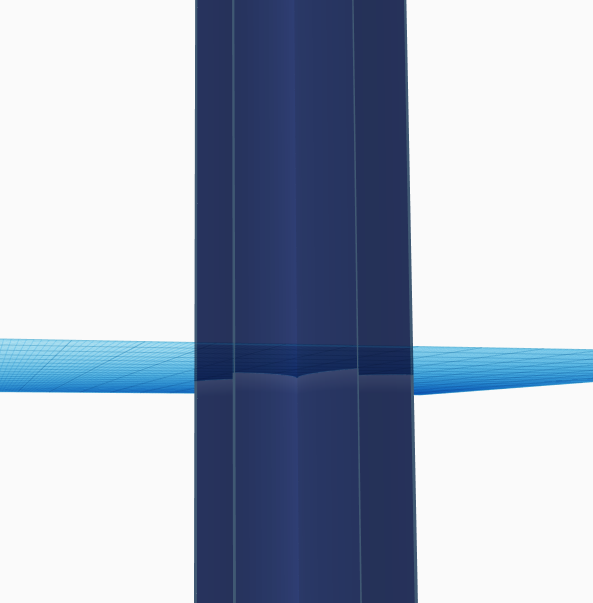
\includegraphics[width=\textwidth]{fithesis/images/flower3D.png} 
    \end{minipage}
  \end{center}
  \caption{The cylinder over the two dimensional "flower" region}
\end{figure}

\begin{definition}
A \textbf{section} of cylinder $Z(R)$ is a set $S$ of points in the form of: $<\alpha, f(\alpha)>$,where $\alpha$ ranges over $R$, and $f$ is a continuous, real-valued function on region $R$. In other words $S$ is graph of $f$ over region $R$.
\end{definition}

\begin{figure}[H]
  \begin{center}
      \begin{minipage}{.4\textwidth}
          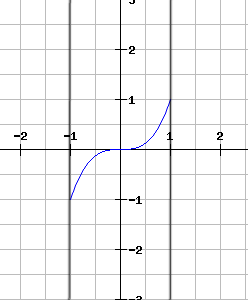
\includegraphics[width=\textwidth]{fithesis/images/section.png}
    \end{minipage}
  \end{center}
  \caption{The $(f)-$section of the cylinder over region from -1 to 1, of the function $f(x) = x^3$}
\end{figure}.

\begin{definition}
A \textbf{$(f_1, f_2)-$sector} of the cylinder $Z(R)$ is a set \^{S} of points in the form of: $<\alpha, \beta>$,where $\alpha$ ranges over $R$, $f_1, f_2$ are the continuous, real-valued functions on region $R$ and for $\beta$ is in range $(f_1(\alpha), f_2(\alpha))$ for $f_1 < f_2$. Where the constant functions $f_1 = -\infty$ and $f_2 = \infty$ are allowed.

In other words $S$ is a (n+1) dimensional space  between $f_1$ and $f_2$ over region $R$.
\end{definition}



\begin{figure}[H]
  \begin{center}
      \begin{minipage}{.33\textwidth}
          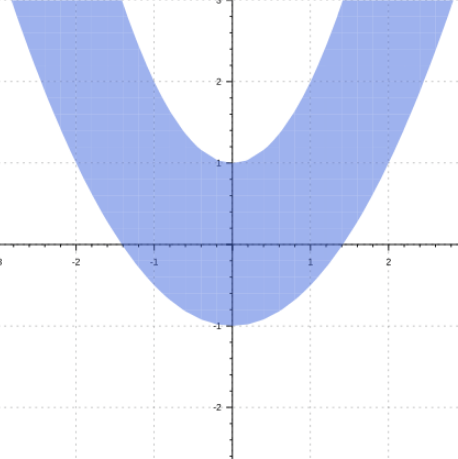
\includegraphics[width=\textwidth]{fithesis/images/sector.png}
    \end{minipage}
  \end{center}
  \caption{The $(f_1, f_2)-$sector of the cylinder two dimensional space, where $f_1(x) = \frac{1}{2}x^2 - 1$ and $f_2(x) = x^2 + 1$}
\end{figure}
Clearly, the sections and sectors of cylinders are also the region and note that if we divide the cylinder of the full-dimensional region into the $(f_1, f_2)-$sectors, this sector is also a full-dimensional region in one higher dimension as an original region. However, if we create  $f$-section of that region, the result region has no volume in a higher dimension.

\begin{definition}{\textbf{Stack over R}}
\newline
Lets be $ f_1 < f_2 \dots < f_n$ ,where $n \in \mathbb{N},\  n \geq 0$ continuous, real-valued functions
defined on $R$,these functions naturally determine decomposition of $Z(R)$ consisting of the following regions:
\begin{itemize}
  \itemsep0em 
    \item the $(f_i,f_{i+1})$-sectors of $Z(R)$ for $0 \leq i \leq n$ . where $f_o =  -\infty$ and $f_{k + 1} =  \infty$
    \item the $f_i$ sections of $Z (R)$ for $1 \leq i \leq n$.
\end{itemize}
    We call such a decomposition a \textbf{stack over $R$} determined by the functions $f_1, \dots f_n$.
\end{definition}

\begin{figure}[H]
  \begin{center}
      \begin{minipage}{0.4\textwidth}
          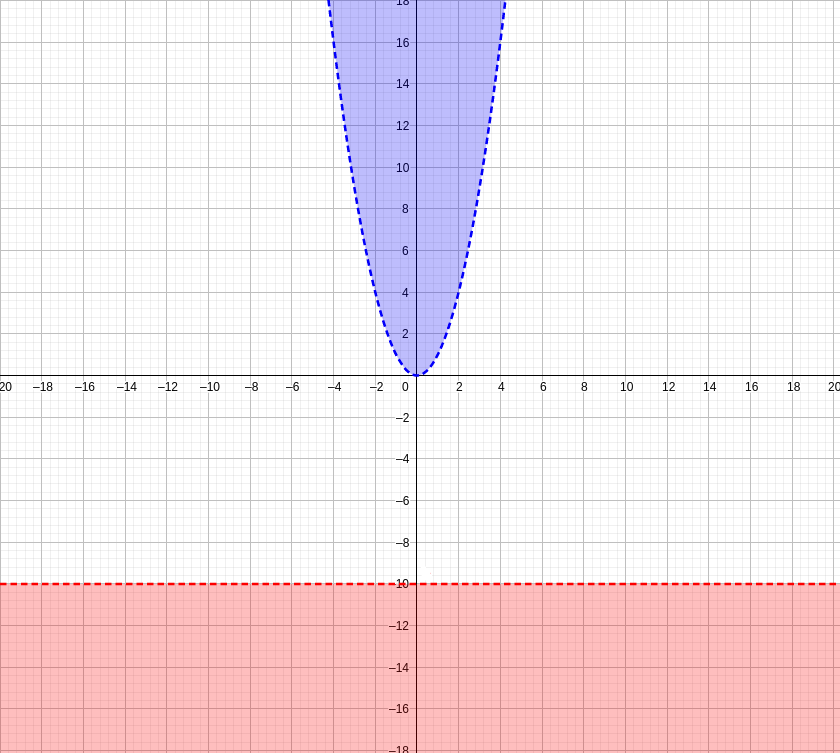
\includegraphics[width=\textwidth]{fithesis/images/stack.png}
    \end{minipage}
  \end{center}
  \caption{The stack determined by the functions $f_1(x) = -10$, $f_2(x) = x^2$, the stack consist of $f_1$, $f_2$ sections and three sectors determinated by $(-\infty, f_1)$, $(f_1, f_2)$, $(f_2, \infty)$}
\end{figure}


\begin{definition}
The decomposition $D$ of $\mathbb{R}^k$ is a \textbf{cylindrical} if either of these conditions holds
\begin{itemize}
  \itemsep0em 
    \item  $k = 1$ and $D$ is a stack over $\mathbb{R}_0$
    \item $k > 1$ and there is a cylindrical decomposition $D'$ of $\mathbb{R}^{k-1}$ such that for each region $R$ of $D'$ some subset of $D$ is a stack over $R$. 
\end{itemize}
\end{definition}


\begin{figure}[H]
  \begin{center}
      \begin{minipage}{0.4\textwidth}
          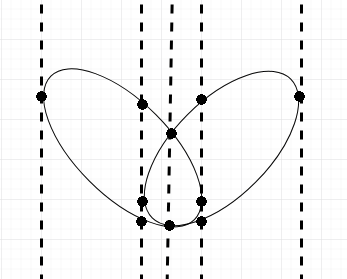
\includegraphics[width=\textwidth]{fithesis/images/cadExample1.png}
    \end{minipage}
  \end{center}
  \caption{The cylindrical decomposition of $\mathbb{R}^2$ consists of eleven stacks. The leftmost stack consists of a single 2-dimensional sector; the next stack consists of
two 1-dimensional sectors and one O-dimensional section (black point); third stack consist of a three 2-dimensional sector and two 1-dimensional sections and so on.}
\end{figure}

After explaining both cylindrical and algebraic decomposition we define \textbf{CAD} of $\mathbb{R}^k$ as a decomposition which is both cylindrical and algebraic.

After defining the CAD problem we want from our algorithm to produce the region, which are sign invariant on the given input. We define now f-invariance of region R


\begin{definition}
Lets be $R$ and $f$ be real valued function defined on $R$ then $f$ is sign invariant on $R$ or $R$ is f-invariant, when one of the following conditions holds:
\begin{itemize}
  \itemsep0em 
    \item $f(\alpha) > 0,\ \alpha \in R$ (f has positive sign in R) 
    \item $f(\alpha) = 0,\ \alpha \in R$ (f has zero sign in R)
    \item $f(\alpha) < 0,\ \alpha \in R$ (f has negative sign in R) 
\end{itemize}
\end{definition}

The region R is then A-invariant, where $A=|A_1\dots A_n|$ and $A_i$ is real valued function defined on $R$, if each $A_i$ is invariant on R.
Collection of the regions is A-invariant if the each element of the collection is A-invariant. As a consequence, we called CAD A-invariant if the result is A-invariant, where A is the collection of input polynomials.

Next in Figure \ref{fig:gingerbreadCAD} we give a more complex example of the CAD. The example is was originally published in \citetitle{LaValle:2006:PA:1213331}. The example shows A-invariant CAD, where A are 4 polynomial functions forming "gingerbread face". In the figure are shown total of 93 CAD regions in total, in which only 37 are full-dimensional.

\begin{figure}
  \begin{center}
      \begin{minipage}{0.7\textwidth}
      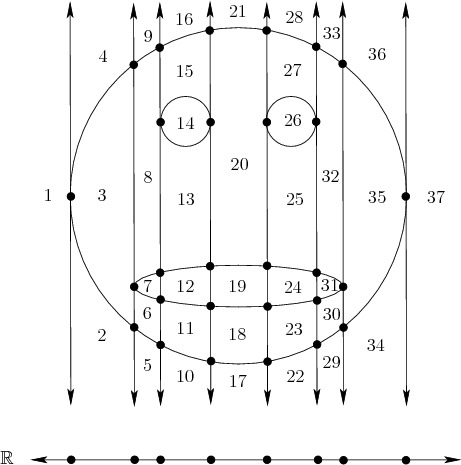
\includegraphics[width=\textwidth]{fithesis/images/CADface.jpg} 
    \end{minipage}
  \end{center}
  \caption{ A cylindrical algebraic decomposition of the gingerbread face. There are $ 37$ $ 2$-cells, $ 64$ $ 1$-cells, and $ 28$ 0-cells. Numbers correspond to open (full dimensional) cells. \cite{LaValle:2006:PA:1213331}}
  \label{fig:gingerbreadCAD}
\end{figure}


\section{Complexity of the algorithm}
As is proven in \citetitle{DAVENPORT198829}

\section{Cylindrical algebraic sub-decomposition}
definition of subcad why subcad complexity in \citetitle{Wilson2014}



\chapter{Algorithm}
TODO elementary description of algorithm, 
\section{Projection phase}
\section{Base phase}
In the base phase of our algorithm, we have to deal with the problem of computing the real roots of a univariate polynomial This problem  could be considered as the fundamental problem of computational algebra\parencite{yap2000fundamental} as well as in many applications ranging from computational geometry to quantifier elimination. 

We decided to solve this problem by implementing real root isolation with the arbitrary precision on the length of intervals. The problem of real root isolation consists of computing intervals with rational endpoints that contain exactly one real root of the polynomial.\parencite{10.1007/11841036_72}

Among many algorithms we decided to implement one based on Descartes's rule of signs together with certain Möbius transformation.

 \subsection{Requirements of Descartes's method}
 The Descartes method requirement for terminating is that input polynomial is square-free.\parencite{ganzha2005computer}
  \begin{definition}
 Given a polynomial $p$ in $R[x]$ where $R$ is a unique factorization domain, $p$ is said to be square-free if $p$ has no divisor (or factor) of multiplicity bigger than one.\parencite{Yun:1976:SDA:800205.806320}
\end{definition}

 Therefore we must ensure this condition before for Descartes's root isolation algorithm. That can be implemented by square-free factorization or polynomial factorization over rational numbers. We implemented both algorithms to see which would have better overall performance in the final implementation.

 The advantages of polynomial factorization are that it provides all the rational roots of a polynomial, which we do not have to find with Descartes's algorithm, but on the other hand, significant advantages of square-free factorization could be its time complexity. In the last chapter, we compare these two algorithms.

 
\subsection{Descartes's method for root isolation}
The advantages of this method are the simplicity of the implementation and a better theoretical upper bound for its computing time on integer polynomials against other techniques such as the Collins-Loos or Heindel's algorithms. 
 For a square-free integral polynomial of degree $n$, we obtain that time complexity of the algorithm belongs to  $O(n^6)$  \parencite{Collins:1976}
 
The basis for our algorithm is Descartes Rule of Signs
\begin{theorem}
[Descartes Rule of Signs]
  Let $p(x) = \sum_{i=0}^n b_ix^i [c, d](x)$ be a non-zero polynomial than $var(b)$ exceeds the number of zeroes of p in the open interval $(c, d)$ by even non-negative integer.\parencite{ganzha2005computer} Where $var(b)$ represents then number of sign changes of $p(x)$
  \end{theorem}
  
This theorem was first mentioned in Descartes's essay The Geometry in 1637 \cite{descartes2007geometry} and later stated and proved in exact form by Gauss in 1828 \cite{gauss1828}. Nevertheless it has two interesting consequences for our algorithm. Primarily if $var(b)$ on interval $ I = (c, d)$ of polynomial $p(x)$ is zero than interval $I$ does not contain any zero of  $p(x)$ and furthermore if $var(b) = 1 $, than $I$ is isolating interval for and contains exactly one root of $p(x)$.

In order to use the consequences in our algorithm we must to know how to transform a polynomial to arbitrary interval.
For this purpose we used Möbius transformation $x \gets \frac{ax + b}{x+1}$  which maps real positive line to interval $(a, b)$. \cite{DBLP:journals/corr/abs-1109-6279} Thus our function for transforming polynomial $p(x)$ is form: 
\begin{equation}
    f(p(x)) =  (x + 1)^n . p(\frac{ax + b}{x+1})
\end{equation}
The next pseudo code of algorithm $DescartesRootIsolation$ combines the  Descartes Rule of Signs theorem and transformation of the polynomial to the arbitrary interval $(a, b)$


\begin{algorithm}[H]
    \SetKwInOut{Input}{Input}
    \SetKwInOut{Output}{Output}
    \Input{
    Univariate polynomial, Lower bound, Upper bound
}
    \Output{Sorted list of all real roots of polynomial}
    
 result $\gets$ emptyList\\
 middleValue $\gets$ $\frac{(upperBound - lowerBound)}{2}$\\
 \If{NumberOfSigneChanges(polynomial) == 0}{
  \Return emptyList
 }
 \If{NumberOfSignChanges(polynomial) == 1 AND
 \newline
 $upperBound - lowerBound < \epsilon $}{
     \Return listOf(middleValue)
 }
 \If{middleValue is root of polynomial}{
    result.append(middleValue)
 }
 leftPoly $\gets$ toInterval(polynomial, lowerBound, middleValue)\\
 rightPoly $\gets$ toInterval(polynomial, middleValue, upperBound)\\
 \Return result $\cup$
 \newline
 DescartesRootIsolation(leftPoly, lowerBound, middleValue) $\cup$
 \newline
 DescartesRootIsolation(rightPoly, middleValue, upperBound)
 \caption{DescartesRootIsolation}
\end{algorithm}

\paragraph{
vytvorenie base cells and indexing
}
\section{Extension phase}

\chapter{Implementation}
The implementation of the algorithm is licensed under MIT License and available in the public GitLab repository of the Faculty of Informatics of Masaryk University. \footnote{
  Available at: \url{https://gitlab.fi.muni.cz/xgeletka/cad}.
} In this chapter, we discuss the implementation details of
the algorithm described previously.

The project is implemented in Kotlin programming language, because of its flexibility, speed of development and further integration with parameter synthesis tool Pithya of the Sybila laboratory located at the Faculty of Informatics of Masaryk University. \footnote{
  Documentation of Pithya available at: \url{https://sybila.fi.muni.cz/tools_html/pithya.html}.
}

\section{Rings library}
Through our project of full-dimensional CAD, we used the implementations from \citetitle{RINGS}. The RINGS is a cross-platform library written entirely in Java language and thus fully compatible with any modern JVM-based language. The library allows to construct different rings and perform arithmetic in them, including both fundamental math operations and advanced methods like polynomial factorization or
linear systems solving\parencite{RINGS}. The whole library is open sourced and licensed under the Apache License, which allows using freely use and modify this library.

We used the library implementation of Rational ring for representing numbers as a fraction of two integers. 
Next, RINGS offer a representation of both univariate and multivariate polynomial rings over a given a ring. We used the implementation of both polynomial rings over the rational numbers and the intergers.
The library also offers a convenient way of generating polynomials, because of its implementation of parser on a given polynomial ring. We used this parser as a useful and cleaner way of building input polynomial for CAD algorithm., instead of building polynomials by an array of polynomial coefficients.



\section{Code structure}
The whole project is divided into four main packages, which correspond to three phases of the CAD algorithm and one package that ties together the functionality of all project and offers public API for full-dimensional CAD. The packages are projection, rootisolation and extension.

\subsection{Projection}
The projection phase of our CAD algorithm is implemented in package \textit{projection}. This package contains abstract class \textit{PolynomialProjection} with the abstract function \textit{project}, which represents the projection of input polynomials into one lower dimension. In this package are also two classes,  which extends this class and implement the abstract projection method. 
We firstly implemented an elementary Collins projection operator in class \textit{BasicPolynomialProjection}. 
Next, we applied changes in Collins operator, which are valid to full-dimensional CAD  recording to \citetitle{STRZEBONSKI2000471}. The changes are implemented in the class FullDimensionalPolynomialProjection, which also extends class PolynomialProjection.
Both classes are using the implemented functionality from the RINGS library. Specifically, we used the library for computing the subresultants of two polynomials and computing derivatives of the polynomial. We also used the implementation of the least recently used cache on already calculated subresultants for saving difficult computational time.

Together with projection classes representing the projection into one lower dimension, we implemented the functions, which represent iterative projection from $n$ dimensional polynomials to univariate polynomials in one dimension. The methods are implemented in the three different classes, which all extend abstract class IterativeProjection. These classes differ in the way they choose the order of variable to project. 
The first class \textit{IterativeProjectionInLastVariable} project the given polynomials always in the last variable with default lexicographic order.
The second class \textit{IterativeProjectionWithGivenOrdering} project iteratively in the given order of polynomial variable.
The third projection \textit{IterativeProjectionWithGreedyChoice} implemented the greedy algorithm, described in \citetitle{Dolzmann:2004:EPO:1005285.1005303}. This greedy algorithm for finding a good admissible projection order follows the idea that we perform the first projection to one lower dimension for all possible variables. Then we determine the sum of total degrees for each single obtained set. We greedily take the best one and repeat like that until there are no variables left to order. Regarding the statistical analysis of this article, it shows that the performance of these orders is
considerably above-average. \parencite{Dolzmann:2004:EPO:1005285.1005303}


\subsection{Root isolation}
The implementation of the root isolation, required in the base and the extension phase of the algorithm, is located in the package root-isolation. This package contains interface of Descarte's root isolation and two implementations of this interface \textit{DescartWithSquareFreeFactorisationRootIsolation} and  \textit{DescartWithPolyFactorisationRootIsolation}.
The implementations differ in the way they satisfy the Descarte's root isolation prerequisite of the square-free polynomial. 
The first implementation uses Yun's algorithm for square-free polynomial factorization implemented in the RINGS library.
The second implementation uses polynomial factorization, which is also implemented in the RING library. Regarding the RINGS library, the implementation of polynomial factorization uses factorization modulo small prime followed by Hensel lifting and naive recombination.

The root isolation of the full-dimensional CAD must also support finding isolating intervals not only for one polynomial but also for the collection of them.
The reason is that we have to precisely compare the relative position of boundaries of the result regions, which are determined by the roots of collection of projected polynomials. It implies that the isolating interval of the projected polynomials cannot be included in themselves or be equal if they are not denoting the same root.
The strategy of iteratively isolate roots of each polynomial does not work because the Descartes algorithms ensure finding disjoint isolating intervals, although the intervals of two different polynomials can overlap.
The first approach, we implemented, is transforming the problem of finding isolating intervals of collection of polynomials to finding isolating intervals of one polynomial. This approach consists of constructing one polynomial, multiplying all polynomials in the input collection and then compute isolating intervals for this polynomial by Descarte's algorithm. 
This simple solution for this problem brings the negative effect in the computational time of the algorithm because the root isolating algorithm then must work with the high degree polynomial.
The second more satisfying approach is to compute the isolating interval with some default precision and then iteratively smaller only these intervals, which are overlapping, while we don't satisfy the condition of disjoint intervals.
We implemented both approaches to compare their computational times in the experimental evaluation.



\subsection{Extension}
The implementation of the extension phase of the algorithm is located in package extension. This package contains class \textbf{\textit{Region}}, which represents the result region of the cad algorithm. The class contains:
\begin{itemize} 
  \item \textbf{the sample point} of the region, representing as a point in $n$ dimensional space. The sample point, as the representant of this region, can be next used to compute sign of input polynomials for this region.
  \item \textbf{the order} of this region concerning the ordering of variables, from the last projected variable to the first. Secondary the order depends on the order of the region in the corresponding dimension; the relative position to other regions in this dimension sets the resulting order, which is then ascending from minus infinity to infinity.
  \item \textbf{the bounds} representing by an array of rational numbers in the corresponding dimension. These boundaries of regions hold only on sample point with coordinates in one lower dimension. This result from the observations that all boundaries are created as a root of projected polynomial evaluated in some sample point in a lower dimension
\end{itemize}
The class \textit{Region} also contains function \textit{extendOverProjection} which return divided region into sign invariant regions in a one higher dimension.

Together with the representation of the result region is in the package extension also located \textit{ExtensionService} which implements iterative extension from one dimension to n dimension over a list of given projections. The service firstly creates the one-dimensional regions and then iteratively calls \textit{extendOverProjection} over all regions in one lower dimension.


\subsection{API of the implemetation}
The class \textit{FullDimensionalCAD} ties together the functionality of all other packages into several overloaded functions.

The overloaded methods take the collection of polynomials over either integers or rational numbers. But in the projection phase, we use only the polynomials over integers. The reason is to save computational time needed with work with the rational numbers and often calling the greatest common divisor used in used function from the RINGS library.
Because of that our API offers input of polynomials over rational numbers, but these methods only convert the polynomials over rational numbers to polynomials over integers, by computing least common multiplier.

Following the principle of reverse control in the implementation of our full-dimensional CAD, we use only the interfaces and then in our API we can easily change the implementations of these interfaces. That allows us to change implementations, which are used through the project and compare their computational time with different input polynomials.

The whole project is fully described with documentation comments for Java programs with links to the articles and the resources, by which we implemented the code.


\section{Check for correctness}
The implementations correctness is verified by unit tests for each class and each package.
We wrote all tests in JUnit framework with total line coverage of the 97 percent.

We tested the root isolation methods on sets of already computed examples. We compare the results from our algorithm with results calculated in the online tool \footnote{
  Available at: \url{https://www.wolframalpha.com/}.
}  and decided if result error satisfies the given precision.
The other two phases of the algorithm, projection, and extension, which are depended on the implementation of the root isolation, we also tested on sets of example on satisfying conditions, which must hold for the defined polynomial projection and the region extension described in Algorithm chapter.

We tested the overall functionality of our implementation, by comparing the results with already computed  decomposition described in \citetitle{Collins:1976} 


\chapter{Experimental evaluation}
\
\section{Comparison to the CAD imlpementations}
\section{Comparison to the sub-CAD imlpementations}

\chapter{Conclusion}

  \printbibliography[heading=bibintoc] %% Print the bibliography.
\end{document}
